\chapter{Fizikai modell}\label{chap:physical_system}

\section{Egyenáramú motor dinamikája}

\begin{figure}[ht]
\begin{center}
\phantomsection{}
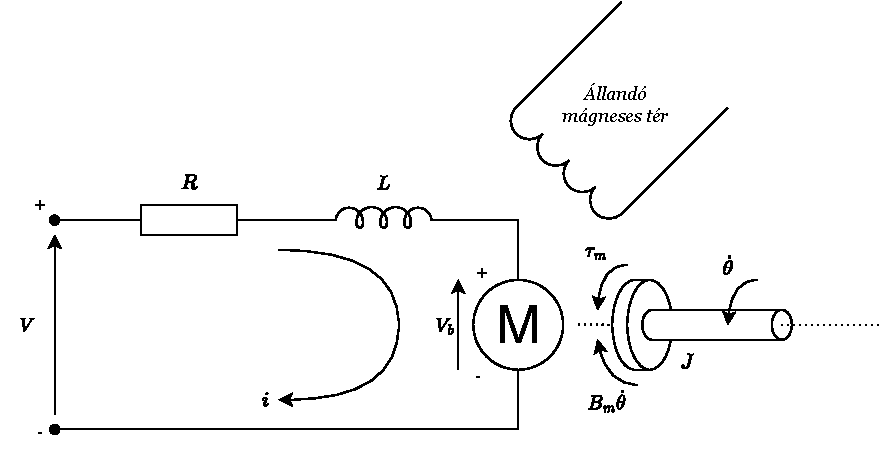
\includegraphics[width=\textwidth]{images/dc_motor_model.pdf}
\caption{Egyenáramú motor áramkör és szabadtest ábra}
\label{fig:dc_motor}
\end{center}
\end{figure}

A robot motorjának modelljét az~\ref{fig:dc_motor}-es ábra mutatja. A felhasznált motor feltételezetten állandó gerjesztésű. A kifejtett nyomaték 
a Biot-Savart-törvény szerint arányos a forgórészen átfolyó árammal. A forgórészben
indukált feszültség pedig arányos annak szögsebességével. A Lenz-törvény alapján 
\begin{align}
    \tau_m = K_\tau i, \\
    V_b = K_e \dot\theta,
\end{align}
ahol $K_\tau$ a nyomatékállandó, $K_e$ a sebesség-feszültség állandó, $\tau_m$ a kifejtett 
nyomaték, $i$ a rotor árama, $V_b$ az rotorban indukált feszültség és $\dot\theta$ a rotor szögsebessége.
Az energia-megmaradás törvénye alapján a két konstans értéke megegyezik
\begin{align}
    K_m = K_\tau = K_e,
\end{align}
így a következőkben $K_m$ paraméterként jelennek meg. A forgórész áramkörére Kirchhoff I. törvénye alapján felírható
\begin{align}\label{eq:armature_circuit}
    V - Ri - L\frac{di}{dt} - K_m\dot\theta = 0,
\end{align}
ahol $R$ a forgórész tekercsének ellenállása, $L$ a tekercs induktivitása, 
$K_m$ a motorállandó, $V$ a motor feszültsége, $i$ a motoráram és $\theta$ a szögelfordulás.
A forgórészt mechanikailag egy merev testként tekintve Newton II. törvénye alapján
\begin{align}\label{eq:rotor_dynamics}
    J\ddot\theta = -B_m\dot\theta + K_m i + \tau,
\end{align}
ahol $J$ a forgórész tehetetlensége, $B_m$ a viszkózus csillapítási együttható, 
$K_m$ a motorállandó, $\theta$ a szögelfordulás, $i$ a motoráram és $\tau$ a forgórészre
ható külső nyomaték. Ez a két lineáris differenciálegyenlet egyértelműen leírja a 
rendszer időtartománybeli viselkedését.
A további vizsgálathoz kedvezőbb a differenciálegyenleteket állapottér modellként felírni.
Egy állapottér modell általánosan
\begin{align}\label{eq:state_space_generic}
    \dot{\bm x} = \bm A \bm x + \bm B \bm u
\end{align}
\begin{align}\label{eq:state_space_generic_out}
    y = \bm C \bm x + \bm D \bm u
\end{align} 
alakban írható fel. 
A két bemenet a külső nyomaték és a motorra adott feszültség. A kimenet a forgórész szöge.
A paramétereket kifejtve~\eqref{eq:armature_circuit} és~\eqref{eq:rotor_dynamics} alapján a modell
\begin{align}\label{eq:state_space}
    \frac{d}{dt}
    \begin{bmatrix}
        \theta \\
        \dot\theta \\
        i
    \end{bmatrix}
    =
    \begin{bmatrix}
        0 & 1 & 0 \\
        0 & -\frac{B_m}{J} & \frac{K_m}{J} \\
        0 & -\frac{K_m}{L} & -\frac{R}{L} \\
    \end{bmatrix}
    \begin{bmatrix}
        \theta \\
        \dot\theta \\
        i
    \end{bmatrix}
    +
    \begin{bmatrix}
        0 & 0 \\
        \frac{1}{J} & 0 \\
        0 & \frac{1}{L} \\
    \end{bmatrix}
    \begin{bmatrix}
        \tau \\
        V \\
    \end{bmatrix}
\end{align}
\begin{align}\label{eq:state_space_out}
    \theta = 
    \begin{bmatrix}
        1 & 0 & 0
    \end{bmatrix}
    \begin{bmatrix}
        \theta \\
        \dot\theta \\
        i
    \end{bmatrix}
    +
    \begin{bmatrix}
        0 & 0
    \end{bmatrix}
    \begin{bmatrix}
        \tau \\
        V \\
    \end{bmatrix}
\end{align}
alakba írható át. A frekvenciatartománybeli vizsgálatokhoz felírható a rendszer 
szög-nyomaték és szög-feszültség átviteli függvénye. Az állapottér modellt felhasználva
\begin{align}\label{eq:transfer_generic}
    \frac{Y(s)}{U(s)} = \bm C{\left(s \bm I - \bm A\right)}^{-1} \bm B + D
\end{align}
általános formában, ahol $\bm I$ az identitás mátrix. Behelyettesítve~\eqref{eq:state_space} és~\eqref{eq:state_space_out}
paramétereit~\eqref{eq:transfer_generic} felírható
\begin{align}\label{eq:transfer_function}
    \begin{bmatrix}
        \frac{\theta(s)}{\tau(s)} \\ 
        \frac{\theta(s)}{V(s)} \\ 
    \end{bmatrix}
    =
    \frac{1}{s\left(JLs^2 + \left(B_m L + JR\right)s + K_m^2 + B_m R\right)}
    \begin{bmatrix}
        Ls + R \\ 
        K_m \\ 
    \end{bmatrix}
\end{align}
alakban.

\section{Egyenáramú motor stabilitása}
A szabályozókör visszacsatoló ágának megbomlása instabilitáshoz vezet, ha a 
szabályozó vagy a szabályozott rendszer önmagában instabil. Ez a valós rendszernél 
szaturációt eredményez, mely a jelen alkalmazás kontextusában nem elfogadható. A motor stabilitása ezért 
egy rendszerkövetelmény, ami a karakterisztikus egyenletből meghatározható.
Az~\eqref{eq:transfer_function}-es átviteli függvény alapján a karakterisztikus egyenlet
\begin{align}
    JLs^2 + \left(B_m L + JR\right)s + K_m^2 + B_m R = 0,
\end{align}
ahol a nullában elhelyezkedő pólussal átszorozva a szögsebesség a vizsgált kimenet.
Ez a polinom valós együtthatókkal rendelkezik, így a Liénard–Chipart kritérium - a Routh-Hurwitz kritérium módosított
alakja - segítségével a stabilitás szükséges és elégséges feltételei
\begin{align}
    JL>0,\quad B_m L + JR > 0,\quad K_m^2 + B_m R > 0.
\end{align}
A feltételekben megjelenő paraméterek mind pozitívak a valós rendszerben, így a rendszer
önmagában aszimptotikusan stabil. Ezen felül linearitásából következik, hogy exponenciálisan stabil.

\section{Irányíthatóság és megfigyelhetőség}
A felhasznált aktuátorok és szenzorok minimalizálása érdekében egy bemenet és egy kimenet használata a cél. 
Az impedancia modell teljes realizálásához további követelmény, hogy a rendszer szögelfordulása és szögsebessége
irányítható legyen a bemeneti feszültség megváltoztatásával, és a szögelfordulás mérésével minden állapot 
megfigyelhető legyen. Az~\eqref{eq:state_space_generic}-os állapottér modell alapján az irányíthatóság feltétele, hogy
\begin{align}
    \left[\begin{array}{c|c|c|c}
        \bm{CB} & \bm{CAB} & \bm C \bm A^2 \bm B & \bm D
    \end{array}\right]
\end{align}
legyen maximális rangú. Behelyettesítve~\eqref{eq:state_space} és~\eqref{eq:state_space_out} paramétereit a kimeneti mátrixot kiegészítve a szögsebességgel
\begin{align}
    \begin{bmatrix}
        0 & 0 & \frac{K_m}{JL} & 0 \\
        0 & \frac{K_m}{JL} & -\frac{K_m\left(B_m L + JR\right)}{J^2L^2} & 0
    \end{bmatrix},
\end{align}
redukált lépcsős alakban
\begin{align}
    \begin{bmatrix}
        0 & 1 & 0 & 0 \\
        0 & 0 & 1 & 0
    \end{bmatrix},
\end{align}
mely mátrix rangja megegyezik sorainak számával, így az irányíthatósági feltétel teljesül. Az előzőekhez hasonlóan a 
megfigyelhetőség feltétele, hogy
\begin{align}
    \left[\begin{array}{c}
        \bm{C} \\ \hline
        \bm{CA} \\ \hline
        \bm C \bm A^2
    \end{array}\right]
\end{align}
legyen maximális rangú, ahol $\bm C$ csupán a szöglfordulást tartalmazza. Ismét behelyettesítve
~\eqref{eq:state_space} és~\eqref{eq:state_space_out} paramétereit
\begin{align}
    \begin{bmatrix}
        1 & 0 & 0 \\
        0 & 1 & 0 \\
        0 & -\frac{B_m}{J} & \frac{K_m}{J}
    \end{bmatrix},
\end{align}
redukált lépcsős alakban
\begin{align}
    \begin{bmatrix}
        1 & 0 & 0 \\
        0 & 1 & 0 \\
        0 & 0 & 1
    \end{bmatrix},
\end{align}
tehát a rendszer minden állapota megfigyelhető a szögelfordulás méréséből.
